%        File: zone-based-update-mechanism-for-lbs_cn.tex
%     Created: Sun Jan 03 01:30 PM 2012 C
% Last Change: Sun Jan 03 01:30 PM 2012 C
%
\documentclass{article}
\usepackage{CJKutf8}

% Package & settings for graphic
\usepackage[pdftex]{graphicx}
\usepackage{subfig} % Enable sub figure
\graphicspath{./figure/}
\DeclareGraphicsExtensions{.png,.jpg,.jpeg,.pdf}

% Package for References & Cite
\usepackage{natbib}

\title{基于区域的LBS更新机制}
\author{Suleiman Almasri, Ziad Hunaiti, Eliamani Sedoyeka and Wamadeva Balachandran}


\begin{document}
\begin{CJK}{UTF8}{gbsn}
	% Make title
  \maketitle

	% Rename
  \renewcommand{\abstractname}{摘要}
	\renewcommand{\figurename}{图}
	\renewcommand{\refname}{参考文献}

	% References style & cite settings
	\bibliographystyle{unsrtnat}
	\setcitestyle{super, square, aysep={}, yysep={;}}

	% Begin content
  \begin{abstract}
		在过去几年中,基于位置服务(Location Based Service,简称LBS)得到快速发展和应用,它方便人们何时何地都能获取到有用的信息。LBS系统通过移动网络,根据移动终端所在位置定位用户,并为用户提供相应的数据和服务。而这样的服务系统往往需要从服务器发送大量的数据给用户,于是本论文提出一个新的更新机制,它可以有效地提升LBS系统的服务性能。同时,该机制将减少网络带宽的使用,从而有利于最大限度地降低用户设备(移动智能手机、PDA等)的内存使用和功率消耗。
  \end{abstract}

  \newpage
  \section{引言}
	随着移动通信和卫星导航的迅猛发展,产生了结合这两个主要技术的新系统,也就是基于位置服务(Location Based Service,简称LBS)系统$1$。LBS系统的基本架构主要有移动设备和移动网络接口两部分,其中移动设备含有以全球卫星导航(Global Positioning System,简称GPS)为主卫星导航接收部件,移动网络接口则通过无线网络与包含一定地理位置信息的服务器相连$2$。LBS系统通过结合智能应用和用户的位置信息,提供相应的服务$3$。该系统已经发展成为人们在途中获取需求信息的一个有用的信息资源提供者。然而,LBS系统性能仍然受组件等缺陷的影响$4$。

	尽管GPS被视为最准确的定位系统,可它仍然存在两个主要缺陷:可用性和百分之百的准确性。而两个缺陷也直接影响到LBS系统的整体性能,尤其是在城市环境下$5$。移动设备是用户获取信息的网关,但不得不承认其存在的几个限制:内存大小、电池寿命和处理器性能,而这三个因数对LBS系统都存在直接的影响$6$。地理信息系统(Geographic Information System,简称GIS)数据库服务器是存储所有用户移动设备访问的信息的主要容器。该数据库的有效管理是非常重要的,必须为其提供一种有效的访问方法,否则可能带来不必要的处理时间和延迟,从而降低整个LBS系统的定位效率$7,8,9$。移动无线网络允许数据在LBS系统和移动设备之间进行传输,然而这种传输方式受到带宽不足的限制,尤其是当很多用户使用该移动网络的情况下$10$。因此,最大限度地减少通过移动网络传输地数据量,可以很大程度地减少延迟和丢包,从而直接提升LBS系统系统。

	\begin{figure}[htbp]
		\centering
		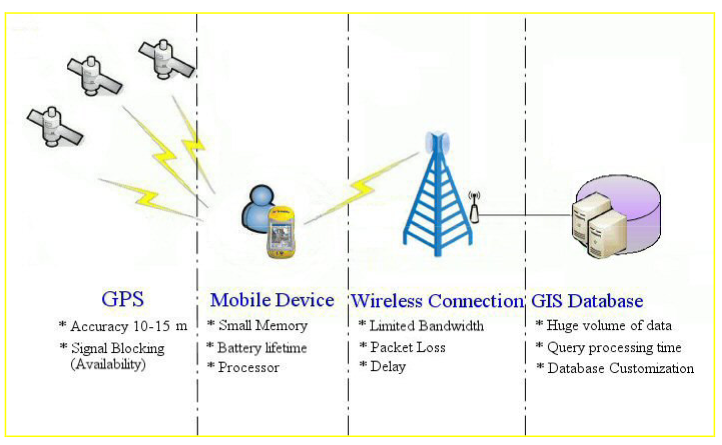
\includegraphics[bb=0 0 722 455, scale=0.45]{figure/fig01.png}
		\caption{LBS的基本架构和它存在的问题}
	\end{figure}

	如果解决上述问题,将有利于提升LBS系统的效率。本论文为GIS数据库管理提出的新机制,就是通过将其划分为若干地理区域来解决上述问题的。通常,LBS系统通过发送一整个较大地理区域相关的大量数据给终端用户以进行信息更新,而通过该方法,最终传输到用户移动设备的数据量将大大减少,这对网络、移动设备和数据库都是非常有利的。现如今,为了提升大型数据库的使用效率以及更好管理,已经在研究开发采用基于区域(比如,更小的地理区域)的策略的LBS系统$11,12$。

	本论文中,基于区域更新策略已被用于测试并探讨它对改善LBS系统性能的影响。我们将区域信息和其对应的数据库划分成两种类型的区域:宏区(Macro-zones)和微区(Micro-zones)。宏区是一个较大的地理区域,例如一个镇。同时,宏区又划分成更小的区域,也就是我们所说的微区(如图\ref{fig:dividing-the-map-into-micro-zones}所示)。

	\begin{figure}[htbp]
		\centering
		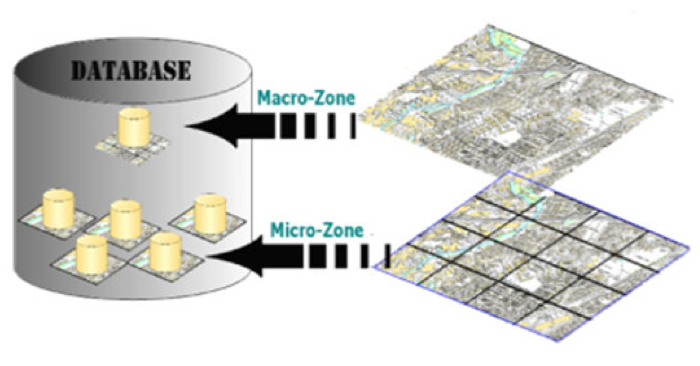
\includegraphics[bb=0 0 700 366, scale=0.45]{figure/fig02.png}
		\caption{将地图细分成微区}
		\label{fig:dividing-the-map-into-micro-zones}
	\end{figure}

	宏区是一个矢量地图。在矢量地图模式中,空间对象通常被投射到一个包含坐标、基准和投影的坐标系中。该空间对象可以是单独的一个点(代表一个人、一辆车或一个喜欢的景点),或者是一条模拟两个点间具有一定联系的直线,也可以是一条代表一系列点之间联系的折线,还可以是一个封闭的多边形(如果该多边形内部有大于180度的角,则称为凸多边形,否则称为凹多边形)$1$。此外,这种宏区还包含用户所在的微区及相邻微区的详细信息。

	微区是一个栅格地图。栅格地图由行和列排列的网格组成,该模式与一张位图图片非常相似,网格中像素点越多,就能获取到更优质的栅格数据$1$。在大多数情况下,栅格图像比矢量图像更加清晰和友好,而用户也更喜欢面对一张好的图像。一个微区的大小被定义成一个行人步行距离以内,例如,一个两公里的距离。为了能缓慢加载与该微区相邻微区的数据信息,每个微区都分配有一个已知的更新点。此外,每个微区都有其唯一的ID和边界,以便在行人到达该微区时自动下载与该微区相关联的数据。用户还可以选择设置该服务为自动下载还是手动下载。

	\section{初期实施和评估}
	为了评估我们提出的新机制,我们选用英国Chelmsford地图的主要部分为实验场景,并采用配有移动GPS扩展的GeoMedia专业GIS系统来进行实验。实施测试前,我们将一台通过HSDPA接到互联网的笔记本电脑(装有GeoMedia专业GIS系统)连接到一端,另一端则通过Holox GPS接收机$13$连接到GPS。实施过程中,我们将Chelmsford矢量地图作为宏区,并细划分成已确定边界的许多微区。配置后的系统将询问用户是否设置为当用户接近相邻微区到一定距离(比如10米)时上传信息到服务器,而且用户还可以选择接受或拒绝消息。如果他(或她)接受,那么将建立一个互联网连接到一台模拟LBS定位的远程服务器。

	在我们于现实世界中测试和应用基于区域的更新机制的过程中,研究人员采用Toshiba Equium笔记本电脑来代替移动终端用户。该笔记本电脑通过蓝牙连接到GPS接受机(Holox BT321)来实现移动终端用户的物理位置。此外,将GeoMedia的专业系统软件作为一个GIS工具来使用。GeoMedia的GPS接收机接收NMEA GPS字符串消息并将其显示在Chelmsford地图上。

	研究人员进行了相应试验以演示该过程。GPS接收机定位用户的位置,进行匹配后通过GeoMedia专业系统标注在地图上。如图\ref{fig:geomedia-fixes-the-user-s-location-using-gps-expansion}所示,当用户在“L区(Zone L)”移动时,GPS接收机也不停地更新该用户的位置。该用户朝北移动。

	\begin{figure}[htbp]
		\centering
		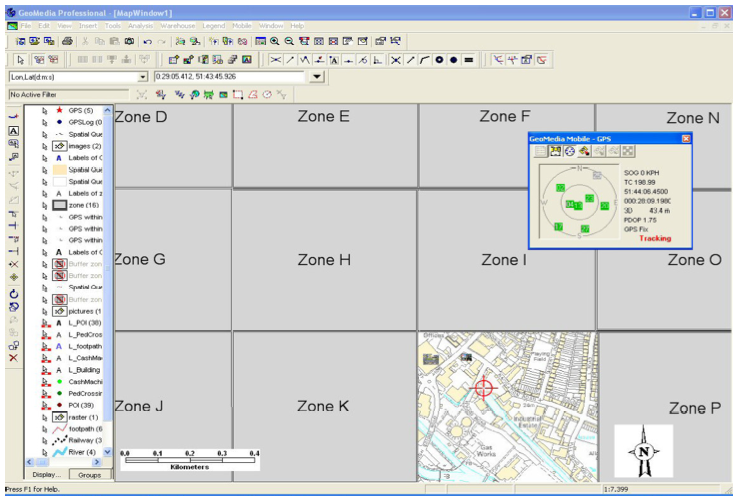
\includegraphics[bb=0 0 738 501, scale=0.45]{figure/fig03.png}
		\caption{采用GPS扩展的GeoMedia定位用户的位置}
		\label{fig:geomedia-fixes-the-user-s-location-using-gps-expansion}
	\end{figure}

	当接近新的微区(I区,Zone L)边界时,系统自动生成一条消息发送给用户,询问是否确认要加载新区域的数据(如图\ref{fig:the-system-asking-the-user-to-load-the-new-zone}所示)。当用户接受该消息后,系统便自动发送新微区的数据到用户的设备中,如图\ref{fig:the-system-loaded-zone-i-into-the-user-s-device}所示。

	\begin{figure}[htbp]
		\centering
		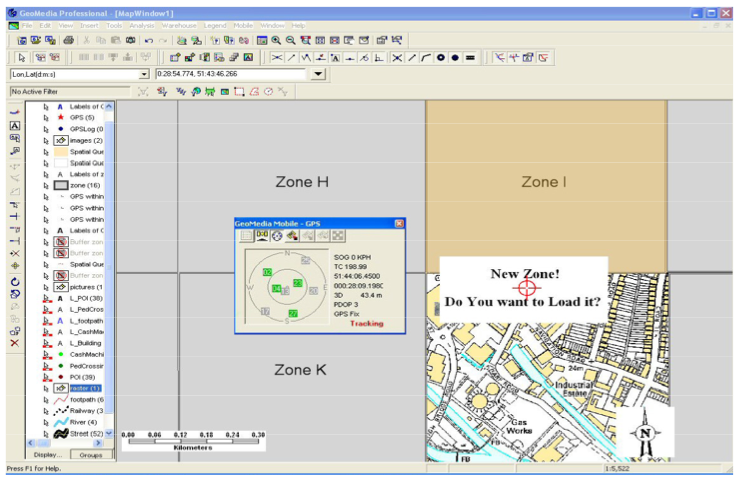
\includegraphics[bb=0 0 740 482, scale=0.45]{figure/fig04.png}
		\caption{系统询问用户是否加载新区域数据}
		\label{fig:the-system-asking-the-user-to-load-the-new-zone}
	\end{figure}

	\begin{figure}[htbp]
		\centering
		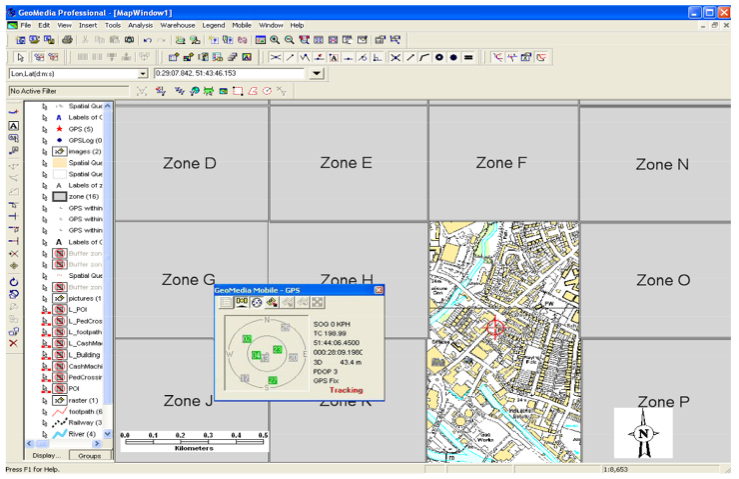
\includegraphics[bb=0 0 739 479, scale=0.45]{figure/fig05.png}
		\caption{系统加载I区的数据到用户的设备中}
		\label{fig:the-system-loaded-zone-i-into-the-user-s-device}
	\end{figure}

	实验的第二部分是观察基于区域更新机制对LBS系统性能的影响,并有效地检测减小地图尺寸对其产生的影响。如图所示,是一个简化的使用网络架构的LBS系统,该系统设在安格利亚鲁斯金大学(Anglia Ruskin University)$11$。本实验主要是为了评估该新的机制在移动连接(延迟、带宽等)和移动设备(内存、电池等)产生的效益。在实验过程中,用两个主要连接在不同环境中进行测试:

	\subsection{高速下行分组接入(High-Speed Downlink Packet Access,简称HSDPA)}
	将Toshiba Equium笔记本电脑通过一张Web “N” Walk PCMCIA无线数据网卡连接到T-Mobile网络,从而建立一个活动的HSDPA(3.5G)无线连接。T-Mobile的 Web “N” Walk数据网卡支持高达1.8Mbit/s的理论速度$10$。

	\subsection{无线局域网(Wireless Local Area Network,简称WLAN)}
	将Toshiba Equium笔记本电脑连接到安格利亚鲁斯金大学的无线局域网,该网络基础设施(IEEE 802.11b)支持54Mbit/s的理论速度。同时,该网络通过使用JANET$14$(一个在英国不同教育机构中使用的网络)以100Mbps的速度连接到互联网。

	为了模拟LBS服务器,将可供搜寻的Chelmsford市主图上传到服务器,不包括该市的微区地图。此服务器可以通过互联网直接访问。在实验过程中,通过使用Ping命令发送ICMP(Internet Control Message Protocol,互联网控制消息协议)包到服务器,来评估服务器在空闲和忙碌状态(下载和上传的时候)下的链路性能。ICMP包通常被用于计算连接请求响应所经历的往返延迟时间(Round Trip Delay Time,简称RTT),从而估计服务在连接环节所产生的延迟时间。此外,在加载主图和区域地图时,会测算时间、功率和内存的利用率等数据,以区分传统系统和基于区域系统的不同。

	\begin{figure}[htbp]
		\centering
		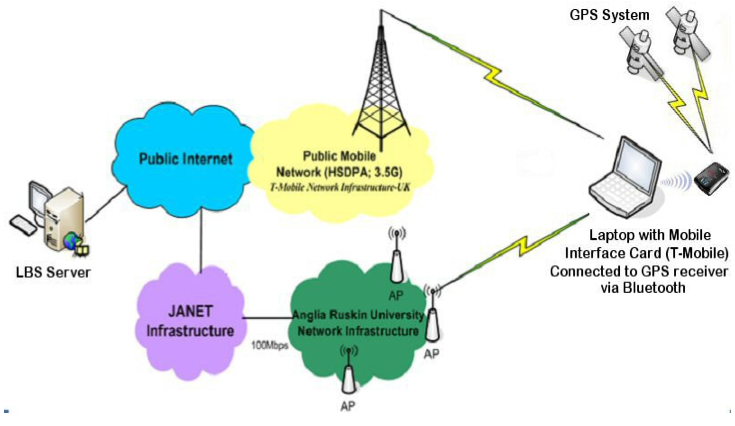
\includegraphics[bb=0 0 735 426, scale=0.45]{figure/fig06.png}
		\caption{实验场景中的网络架构}
		\label{fig:network-architected-for-experimental-scenarios}
	\end{figure}


	\section{实验结果}
	实验中进行了三项任务的设计。其中第一个就是衡量在不同的网络连接类型下,下载地图(包括Chelmsford主图和微区图)所需时间,该任务获得的结果如图\ref{fig:the-time-taken-to-load-maps}所示。从结果分析可知,在两种不同网络连接类型下,下载全图所需时间都约为下载区域图所需时间的四倍:在HSDPA连接情况下,完整下载全图到用户设备所需时间为256.83秒,而对于区域地图而言,只需62.56秒;在WLAN连接情况下,完整下载全图所需时间为183.78秒,而区域地图只需46.88秒。因此,基于区域的更新机制能够有效减少数据的拥塞,也减少了访问网络所需时间,从而直接地提升了移动网络地性能。

	\begin{figure}[htbp]
		\centering
		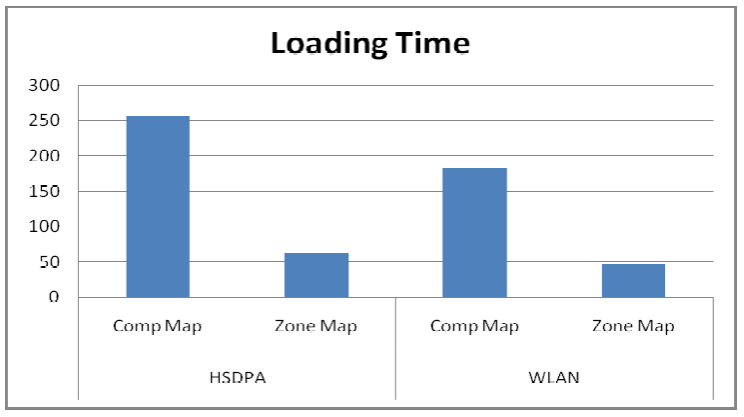
\includegraphics[bb=0 0 744 417, scale=0.45]{figure/fig07.png}
		\caption{在使用HSDPA和WLAN无线连接情况下,加载完整地图和小地图所需时间}
		\label{fig:the-time-taken-to-load-maps}
	\end{figure}

	第二个实验任务便是衡量移动设备和LBS服务器之间地延迟。如图\ref{fig:the-rtt-taken-to-send-icmps}所示,该测试在四个不同的环境下重复进行:
	\begin{enumerate}
		\item 在HSDPA连接下的空闲状态
		\item 在HSDPA连接下的下载状态
		\item 在WLAN连接下的空闲状态
		\item 在WLAN连接下的下载状态
	\end{enumerate}
	
	如之前所提到的,通过使用Ping命令发送ICMP包到服务器,来评估服务器在空闲和忙碌状态(下载和上传的时候)下的链路性能。ICMP包通常被用于计算连接请求响应所经历的RTT,从而估计服务在连接环节所产生的延迟时间。

	在用户访问网络(下载地图)的时候,将产生较大的延迟。然而,基于区域的更新机制减少了大量数据在服务器和移动设备之间的传输,从而降低了移动网络带宽的需求和访问移动网络的时间开销。所以,使用小地图代替大地图,可以显著地降低在网络上的开销。

	\begin{figure}[htbp]
		\centering
		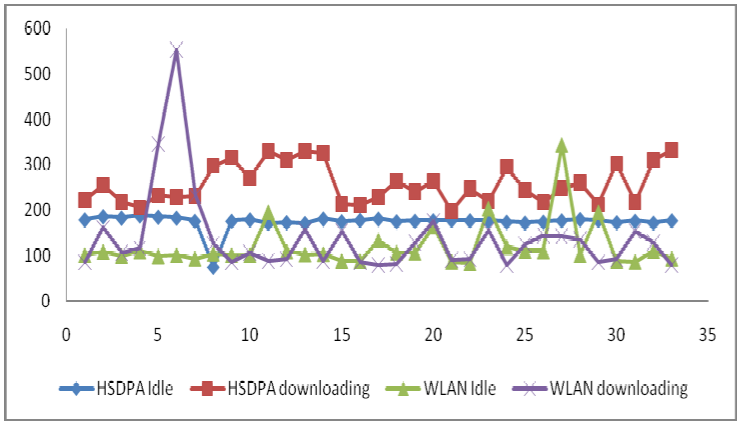
\includegraphics[bb=0 0 743 426, scale=0.45]{figure/fig08.png}
		\caption{在空闲和下载状态下,发送ICMP到服务器所需RTT}
		\label{fig:the-rtt-taken-to-send-icmps}
	\end{figure}

	第三个实验任务是衡量笔记本电脑的用电率,而这是通过监测电池在以下两种情况下完成的:
	\begin{enumerate}
		\item 空闲模式(没有运行大型耗电应用)
		\item 下载模式(下载地图)
	\end{enumerate}

	如图\ref{fig:the-laptop-battery-discharge-rate}所示,在下载模式下,电池用电非常快,而在空闲模式下或者没有接收数据的情况下则较少。

	\begin{figure}[htbp]
		\centering
		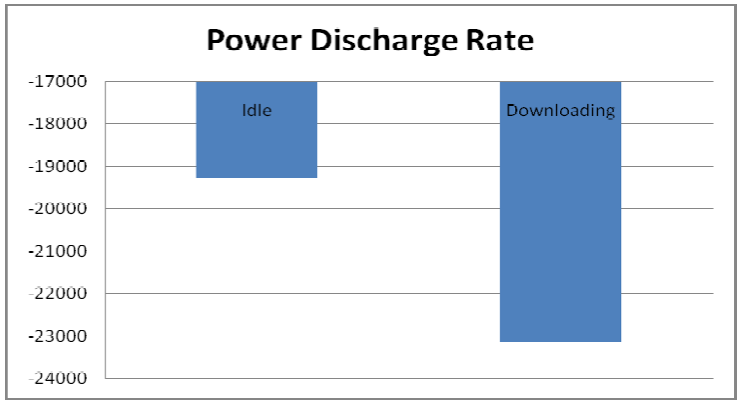
\includegraphics[bb=0 0 741 406, scale=0.45]{figure/fig09.png}
		\caption{在空闲和下载模式下,笔记本电脑的用电率}
		\label{fig:the-laptop-battery-discharge-rate}
	\end{figure}

	从获得的结果显然可知,基于区域的更新机制直接影响移动设备的性能。这还可以通过比较不同情况(下载整张地图和区域地图)下的功耗得出,图\ref{fig:the-calculated-total-battery-discharge-rate}所示为分别针对整张地图和小地图所计算得到的总的电池用电率。基于区域的机制可以让移动设备的电池使用寿命更长,而这在紧急情况中用户无法为设备充电的情况下,是非常有利的。同时,该机制还有利于用户更好地利用和管理设备的存储空间,这点对存储能力非常有限的移动设备是非常重要的。基于区域的机制使得用户得益于LBS服务的同时,还可使用占用一定内存的其它应用。此外,对于一个较小的数据库,它可以更快地响应用户的查询请求。

	\begin{figure}[htbp]
		\centering
		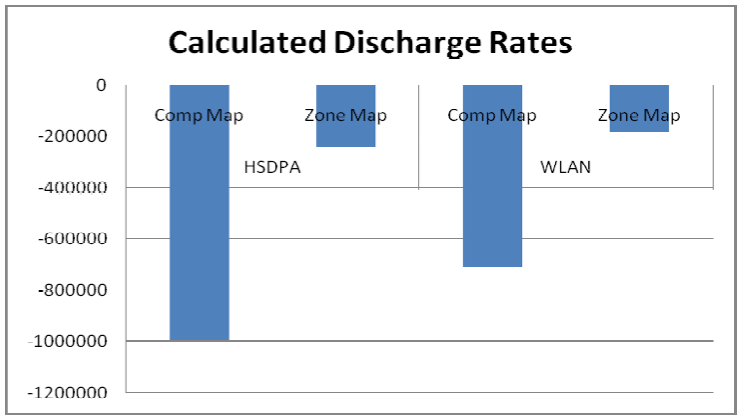
\includegraphics[bb=0 0 744 419, scale=0.45]{figure/fig10.png}
		\caption{在分别下载整张地图和小地图的情况下,计算得到的总的电池用电率}
		\label{fig:the-calculated-total-battery-discharge-rate}
	\end{figure}


	\section{结论和进一步的工作}
	本论文研究讨论了基于区域的策略以提升LBS定位性能。一个原型系统也已经得到了实施和评估。从这项研究工作中取得的成果表明,这一机制已经为减少信息量做出了重大贡献。此外,这种机制最大限度地减少了可能由终端用户上传冗余信息造成的不必要开销,而这为整个LBS系统提升了性能。这一机制的全面实施需要进行更全面的评估,并用新的系统进行测试。


	\section{感谢}
	本研究工作受鹰图有限公司(全球领先的空间信息管理软件的先驱)赞助,在其注册研究实验室计划下进行。地图由地形测量局提供。最后,感谢Ralph Diment(英国Intergraph公司)和Chris Philips(全国地形测量局)的帮助和支持。

	% Import references datas
	\bibliography{references.bib}

	\end{CJK}
\end{document}
